\chapter{Paradigma orientado a objetos}

\label{ch:poo}

% -----

Uno de los debates principales sobre JavaScript es su soporte hacia el paradigma orientado a objetos. Existe una amplia gama de opiniones y posturas con respecto a JavaScript y su uso dentro de dicho paradigma. Las opiniones pueden ir desde la negativa, es decir, que no lo soporta, hasta la positiva, pasando por un intermedio de que tiene cierto soporte, pero no naturalmente.

En éste capítulo se buscará realizar un análisis sobre características típicas del paradigma orientado a objetos, tratándo de ver de qué manera llega JavaScript a éstas características.

% -----

\section{Clases}
\label{clases}

Previo a la salida de ES6 (es decir, en la version 5 de JavaScript) la creación de clases en JavaScript se realiza mediante el uso de patrones para la creación de objetos. La realidad es que en JavaScript no existe un soporte formal o natural para las clases, sino que hay que recurrir a estos patrones para simularlo. Los más populares, a mi entender, son:

\begin{itemize}
	\item Factory class pattern
	\item Functional class pattern
	\item Prototype class pattern
\end{itemize}

\subsection{Factory class pattern}

Se trata de una función de tipo \textit{factory} (fábrica) utilizada para crear elementos u objetos, con ciertas propiedades y bajo cierto comportamiento. En nuestro caso, dicha función será quien cree nuestras nuevas instancias de lo que queremos moldear como clase.

\begin{lstlisting}[title={Factory class pattern}]
function animalFactory(nombre) {
  var temporal = {};
  temporal.nombre = nombre;
  temporal.saludar = function() {
    console.log("Hola, soy "+this.nombre)
  };

  return temporal;
}

var gato = animalFactory("Garfield");
var perro = animalFactory("Oddie");

gato.saludar();		// Hola, soy Garfield
perro.saludar();	// Hola, soy Oddie
\end{lstlisting}

Si bien puede resultar un poco confuso al principio, para quienes estén acostumbrados al patrón Factory, este ejemplo quizás resulte más trivial. A simple vista, la única \textit{ventaja} es que no se necesita usar \code{new} a la hora de realizar la instanciación de nuevos objetos. 

Para el objetivo que buscamos, que es simular el soporte de clases, este patrón es útil.

\subsection{Functional class pattern}

Este patrón también es conocido como Constructor pattern. Aprovechando el uso de la palabra \code{new}, podemos omitir la creación de un objeto temporal dentro de nuestra función. De hecho, la palabra \code{new} no solamente crea un nuevo objeto (instancia), sino que además establece quién fue la función de construcción (se puede pensar como "`de quién hereda el objeto"').

\begin{lstlisting}[title={Functional class pattern}]
function Animal(nombre) {
  this.nombre = nombre;
  this.saludar = function() {
    console.log('Hola, soy ' + this.nombre);
  };
};

var gato = new Animal('Garfield');
var perro = new Animal('Oddie');

gato.saludar();		// Hola, soy Garfield
perro.saludar();	// Hola, soy Oddie
\end{lstlisting}

Notar las diferencias con el ejemplo del Factory Pattern. Por un lado, el uso del \code{this} dentro de la función y la falta de necesidad de retornar el objeto (esto sucede implícitamente gracias al \code{new}). Por otro lado, a la hora de crear instancias es importante utilizar la palabra \code{new}.

Un detalle muy importante a tener en cuenta tanto en éste patrón como en el Factory pattern: Para cada instancia creada, la misma poseerá una copia del código de \code{saludar()} en memoria. Parece un detalle menor, pero supongamos que en vez de un solo método, nuestra clase tiene varios, y que ademas precisamos generar una gran cantidad de instancias, significaría estar desperdiciando espacio en memoria.

También para tener en cuenta: No existen reglas ni restricciones sobre los nombres de las funciones constructoras, pero existe una convención entre los programadores de usar la letra capital en los nombres de las funciones constructoras (esto es, que la primera letra sea mayúscula).

\subsection{Prototype class pattern}

Para tratar de resolver el problema recién mencionado, en donde cada instancia tiene una copia del código de la función, es necesario hacer un buen uso del concepto de prototipo en JavaScript, el cual se hizo mención en la sección \ref{sec:prototype}.

\begin{lstlisting}[title={Prototype class pattern}]
function Animal(nombre) {
  this.nombre = nombre;
}

Animal.prototype.saludar = function() {
  console.log('Hola, soy ', this.nombre);
};

var gato = new Animal('Garfield');
var perro = new Animal('Oddie');

perro.saludar(); 	// Hola, soy Garfield
gato.saludar(); 	// Hola, soy Oddie
\end{lstlisting}

Para este caso, tendremos una función constructora \code{Animal}, la cual estará vinculada a su \code{[[Prototype]]}, un objeto que contendrá entre sus propiedades, a la función \code{saludar}. Bajo este patrón, nos obviamos de que cada instancia tenga una copia de la función saludar, y que gracias a la "`cadena del prototipo"' ese comportamiento esté delegado en \code{Animal.prototype}.

\subsection{\code{class} en ES6}
\label{clasesenes6}

A partir de la versión ES6, una de las características más jugosas es la del uso de la palabra reservada \code{class}. Para desgracia del lector, ésta introducción al lenguaje no es más que \textit{syntactic sugar}. Mediante una sintaxis más amena y amigable se alcanza la creación de clases, pero en el fondo la semántica es idéntica al Prototype class pattern.

\begin{lstlisting}[title={Ejemplo de \code{class}}]
class Animal {
  constructor(nombre) {
    this.nombre = nombre;
  }
  saludar() {
    console.log('Hola, soy ', this.nombre);
  }
}

var gato = new Animal('Garfield');
var perro = new Animal('Oddie');

perro.saludar(); 	// Hola, soy Garfield
gato.saludar(); 	// Hola, soy Oddie
\end{lstlisting}

\section{Herencia}
\label{herencia}

Como se ha mencionado anteriormente, JavaScript tiene la particularidad de tener la herencia prototipada en vez de la herencia clásica. Este tipo de herencia es bastante poderosa, aunque también a veces incomprendida y mal aplicada.

\subsection{Herencia simple mediante \code{prototype}}

La herencia prototipal es tan potente que, haciendo un esfuerzo y algunos artilugios, se podrá simular la herencia clásica. La diferencia entre estos dos tipos de herencia es que en la herencia clásica, las subclases poseen una copia del comportamiento de clases. En la herencia prototipal no existe este concepto de copia. Un objeto tiene un prototipo y en caso de que el objeto no tenga un atributo o método necesario, delegará esta responsabilidad a su prototipo. Ésto se llama delegación de comportamiento.

Ahora, supongamos el siguiente código:

\begin{lstlisting}[title={Analizando herencia prototipal en JS}]
function Vehiculo(tipo) {
  this.tipo = tipo;
}

Vehiculo.prototype.mostrarTipo = function() {
  console.log(this.tipo);
}

function Auto(marca) {
  Vehiculo.call(this, "terrestre");
  this.marca = marca;
}

Auto.prototype = Object.create(Vehiculo.prototype);
Auto.prototype.constructor = Auto;

Auto.prototype.mostrarMarca = function () {
  console.log(this.marca);
}

var fitito = new Auto("Fiat");
var falcon = new Auto("Ford");
 
fitito.mostrarMarca();      // Fiat
fitito.mostrarTipo();       // terrestre

falcon.mostrarMarca();      // Ford
falcon.mostrarTipo();       // terrestre
\end{lstlisting}

Tal como se mencionó en la sección \ref{clases}, las funciones en JavaScript son un mecanismo por naturaleza para \textit{simular} las clases. ?`Qué sucede en el código de arriba? Se definen las funciones \code{Vehiculo} y \code{Auto} que serán nuestras clases. Ambas funciones actúan de constructoras. Al \code{[[Prototype]]} de \code{Vehiculo} se le agrega un método \code{mostrarTipo} mientras que al \code{[[Prototype]]} de \code{Auto} se le agrega \code{mostrarMarca}. Hasta ese punto es fácil de entender lo sucedido si se ha comprendido las secciones de prototype y de clases. 

?`Qué pasa en las líneas 10, 14 y 15? 
\begin{itemize}
\item Para el caso de la línea 10, la sentencia \code{Vehiculo.call(this, "terrestre")} está simulando una llamada al constructor padre. Lo que sería análogo a hacer \code{super} en Java. Ésta es una de las partes más feas del código, ya que esta llamada debe ser de forma manual, y dándo como parámetro el contexto del invocador.
\item En la línea 14 estamos "`pisando"' el viejo objeto \code{Auto.prototype} que había sido creado al momento de declarar la función \code{Auto}, y creando un nuevo objeto. El método \code{Object.create} crea un nuevo objeto y establece como prototipo del objeto lo que haya sido pasado como primer argumento de la función.
\item La línea 15 es la que quizás muchos programadores suelen omitir. Sin ella, si hacemos \code{console.log(fitito)} o \code{console.log(fitito.constructor)} podemos verificar que nos figura que \code{fitito} es \code{Vehiculo} en vez de \code{Auto}. ?´Por qué sucede esto? En la línea 14, cuando hicimos la vinculación del prototype de \code{Auto} con el prototype de \code{Vehiculo}, creamos un nuevo objeto y hemos perdido la referencia de \code{Auto.prototype.constructor}.
\end{itemize}

En ejecución, podemos imaginarnos la siguiente imagen como una representación de lo que hay en memoria:

\newpage

\begin{figure}[H]
\centering
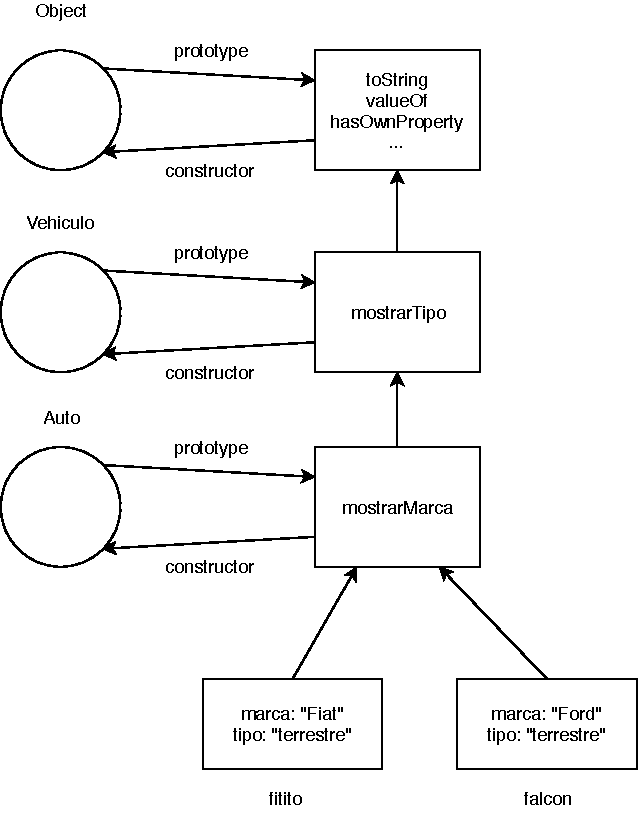
\includegraphics{Figures/Herencia}
\decoRule
\caption[Herencia prototipada]{Diagrama del código presentado}
\label{fig:herencia}
\end{figure}

\subsection{\code{extends} en ES6}

Tal como se explicó sobre la palabra reservada \code{class} en la sección \ref{clasesenes6}, otra de las características que se introdujeron a partir de la versión ES6 es la de la palabra \code{extends} para simular la herencia de clases. Nuevamente ocurre lo mismo que lo mencionado anteriormente: Esta característica es meramente \textit{syntactic sugar} que le omite al programador la necesidad de pensar en prototipos. 

\begin{lstlisting}[title={\code{extends} en ES6}]
class Vehiculo {
  constructor(tipo) {
    this.tipo = tipo;
  }
  mostrarTipo() {
    console.log(this.tipo);
  }
}

class Auto extends Vehiculo {
  constructor(marca) {
    super("terrestre");
    this.marca = marca;
  }
  mostrarMarca() {
    console.log(this.marca);
  }
}

var fitito = new Auto("Fiat");
var falcon = new Auto("Ford");
     
fitito.mostrarMarca();      // Fiat
fitito.mostrarTipo();       // terrestre

falcon.mostrarMarca();      // Ford
falcon.mostrarTipo();       // terrestre
\end{lstlisting}

Para el programador que viene de C++ o Java, este uso de \code{class} y \code{extends} es, por lejos, muchísimo más amigable que crear funciones y vincularlas mediante sus prototipos. Otra de las introducciones a partir de ES6 es el uso del \code{super} en el constructor. Esto facilita enormemente la llamada al constructor de la superclase, o de métodos de la superclase, además de mimetizar la sintaxis de Java. 

\subsection{Herencia múltiple}

Dado que los objetos "`heredan"' de un único prototipo, el lenguaje no provee ninguna herramienta natural para el soporte de la herencia múltiple. Otros lenguajes buscan alcanzar la herencia múltiple mediante el uso de interfaces. En JavaScript no existen las interfaces, pero sí existe una técnica llamada mixins (acrónimo para \textit{mixed in}, del inglés "`mezclado"') para introducir un comportamiento a una clase sin necesidad de hacerla heredar de otra.

Una función de Mixin suele tener esta forma:

\begin{lstlisting}[title={Función de Mixin}]
function mixin(fuente, destino) {  
  for (var prop in fuente) {
    if (fuente.hasOwnProperty(prop)) {
      destino[prop] = fuente[prop];
    }
  }
}
\end{lstlisting}

Lo ideal sería pensar en \code{fuente} como un objeto cuyas propiedades serán los miembros a "`inyectar"' en \code{destino}. Esta técnica llevó al estándar a agregar un método \code{Object.assign} a partir de ES6, el cual copia los valores de todas las propiedades enumerables en un objeto destino.

Otra manera de implementar los Mixins en ES6 es aprovechando que las clases son de primer órden. Éstas pueden ser pasadas como argumento o ser retornadas por una función.

\begin{lstlisting}[title={Haciendo uso de \code{class} como expresión}]
var MyMixin = (superclass) => class extends superclass {  
  saludar() {
    console.log('hola!');
  }
};

class Foo {}
class Bar extends MyMixin(Foo) {
  despedirse() {
    console.log('chau!');
  }
}

var objeto = new Bar();

objeto.saludar();			// hola!
objeto.despedirse();	// chau!
\end{lstlisting}

Como se puede observar, existen varias formas de aplicar esta técnica. Como se mencionó anteriormente, no hay soporte para herencia múltiple en JavaScript, aunque ésta es una forma de resolver el problema. Aún así, tiene sus defectos. El \textit{shadowing} u \textit{overriding} de métodos con el mismo identificador es una convención a tener en cuenta. También hay que pensar en el costo, ya que copiar las propiedades de un objeto a otro requiere de un esfuerzo.

\section{Encapsulamiento}

Dependiendo la perspectiva, se puede decir que el lenguaje tampoco provee un mecanismo natural para el encapsulamiento. Si hablamos de ocultar el estado de un objeto, es decir, de hacer sus datos miembro privados, no existe ninguna palabra reservada para ello. De hecho, todas las propiedades de un objeto son públicas.

Existe una convención extra oficial de que los miembros privados de un objeto comiencen su identificador con un guión bajo. Nuevamente, ésta no es una convención del lenguaje, sino de la comunidad. Más allá de la convención, volvemos a lo mismo: Por fuera se puede analizar cuál es el valor ligado a dicha propiedad.

\begin{lstlisting}[title={Descubriendo variables "`privadas"'}]
class Persona {
  constructor(nombre, saldo) {
    this.nombre = nombre;
    this._saldo = saldo;
  }
}

var pepe = new Persona('Jose', 25);

console.log(pepe.nombre);	// Jose
console.log(pepe._saldo);	// 25
\end{lstlisting}

Como se puede observar en el ejemplo, se busca hacer privada la propiedad \code{\_saldo}, pero sin embargo es visible desde afuera del objeto.

Por suerte mediante el uso de \textit{closures}, se puede lograr el encapsulamiento, pero solo mediante el uso de funciones constructoras. Lamentablemente, para la sintaxis de \code{class} de ES6 no hay soporte nativo aún. Al momento de escribirse este documento, existe una propuesta en borrador para agregar al lenguaje, la cual se encuentra en \textit{Stage 3} (para más información, ver \href{https://github.com/tc39/proposal-class-fields#private-fields}{https://github.com/tc39/proposal-class-fields\#private-fields}).

\begin{lstlisting}[title={Alcanzando variables privadas mediante closures}]
function Persona(nombre, saldo) {
  var saldoPrivado = saldo;
  this.nombre = nombre;
  this.obtenerSaldo = function() {
    return saldoPrivado;
  }
  this.actualizarSaldo = function(nuevoSaldo) {
    saldoPrivado = nuevoSaldo;
  }
}

var pepe = new Persona('Jose', 25);

console.log(pepe.nombre);					// Jose
console.log(pepe.saldoPrivado);		// undefined
// OK, ya que es una propiedad privada.
console.log(pepe.obtenerSaldo());	// 25
pepe.actualizarSaldo(32);
console.log(pepe.obtenerSaldo());	// 32
\end{lstlisting}

Un detalle menos obvio pero aún así importante, es que necesariamente los \textit{setters} y \textit{getters} de las variables ocultas por el closure deberán formar parte de la función constructora (es decir, no podrán definirse dentro del prototipo), lo que significa nuevamente que cada instancia de \code{Persona} tendrá código repetido, lo que implica gasto en memoria. Bajo esta situación, nos encontramos en un \textit{trade-off} de tener datos miembro privados, pero no poder hacer uso correcto del patrón prototipal.


\section{Polimorfismo}

Quizás uno de los puntos más complicados de analizar en cuanto a JavaScript y su relación con el paradigma de orientación a objetos sea el de polimorfismo, dado que por su naturaleza de débilmente tipado y su particularidad de herencia prototipada, no resultará simple hacer una comparación con lenguajes como C++ o Java. 

Para el caso de las funciones "`polimórficas"' el lenguaje no pone restricciones en relación a la aridad ni el tipo de los parámetros. Si la cantidad de argumentos dados al momento de una invocación es menor a la cantidad de parámetros formales de la función, entonces los restantes se considerarán con valor \code{undefined}. 

Existe un identificador especial reservado para el vector de argumentos en JavaScript, bajo el identificador de \code{arguments}. Este es un objeto especial, aunque a simple vista parece un arreglo, no lo es. Funciona de una forma similar a lo que es \code{args} en Java o \code{argv} en C++. Supongamos a continuación una función que no tiene definidos parámetros formales, pero aún así recibe argumentos a la hora de invocarla.

\begin{lstlisting}[title={Analizando \code{arguments}}]
function mostrarArgumentos() {
  for (var i = 0; i < arguments.length; i++) {
    console.log(i + ". " + arguments[i]);
  }
}

mostrarArgumentos("hola", 1, true, { a: 3 });

// 0. hola
// 1. 1
// 2. true
// 3. [object Object]
\end{lstlisting}

Para el caso de polimorfismo bajo una misma jerarquía de herencia, dado que el lenguaje es débilmente tipado, no posee las restricciones fuertes que posee un lenguaje como Java. Al ser interpretado, no existe un chequeo estático para corroborar que un método que esté siendo invocado pertenezca a un tipo o una clase particular. Ésta característica, la de redefinir un método de la superclase en una subclase, se llama polimorfismo de inclusión (o de subtipado).

\begin{lstlisting}
class Animal {
	mover() {}
}
class Pez extends Animal {
  mover() {
    console.log("Soy pez y estoy nadando...");
  }
}
class Ave extends Animal {
  mover() {
    console.log("Soy ave y estoy volando...");
  }
}

var animales = [new Pez(), new Ave()];

for (let animal of animales) {
  animal.mover();
}

// Soy pez y estoy nadando...
// Soy ave y estoy volando...
\end{lstlisting}

?`Qué sucede exactamente?. En ejecución, cada elemento de la lista de \code{animales} hará búsqueda del método \code{mover} en su cadena de prototipo. En caso de no encontrarlo, resultará en un error en ejecución. 

\section{Modularidad}
\label{sec:modulos}

Durante sus primeros 20 años de vida, JavaScript no proveía soporte para módulos de una forma nativa. En 2015 con la salida de ES6, el lenguaje adquirió ese soporte nativo que le faltaba. Sin embargo, aún no todos los navegadores (o motores) soportan todas las funcionalidades introducidas en ES6 y las nuevas versiones del estándar.

En ésta sección vamos a mencionar cuáles son las formas en las que se alcanza la modularidad en JavaScript.

\subsection{Módulos mediante patrones}

Al igual que sucede con las clases, se hace el uso de IIFE y closures para aplicar patrones conocidos en la creación de módulos. El patrón por excelencia en este caso es el Revealing Module pattern. Si este patrón es implementado mediante IIFE, se lo puede pensar al módulo como un singleton, ya que al momento de definir el módulo se está creando una única instancia del mismo.

\begin{lstlisting}[title={Revealing module pattern}]
var ModuloSaludador = (function () {
  var cantidadSaludos = 0;

  var incrementarSaludos = function() {
    cantidadSaludos++;
  }

  var saludar = function() {
    console.log("hola");
    incrementarSaludos();
  }

  var despedirse = function() {
    console.log("chau");
    incrementarSaludos();
  }

  var mostrarContador = function() {
    console.log(cantidadSaludos);
  }

  return {
    saludar: saludar,
    despedirse: despedirse,
    imprimirEstado: mostrarContador
  }
}());

ModuloSaludador.saludar();				// hola
ModuloSaludador.despedirse();			// chau
ModuloSaludador.imprimirEstado();	// 2
\end{lstlisting}

Para el ejemplo dado, se mantiene un estado interno que cuenta la cantidad de saludos dados. Se puede apreciar como tanto \code{cantidadSaludos} y la función \code{incrementarSaludos} son de alguna forma atributos privados del módulo. 

Lo que retorna la función constructora del módulo en realidad es un objeto con las funciones del mismo, a modo de API. Notar el detalle de la función \code{mostrarContador}, que internamente para el módulo se llamará de esa manera, pero el módulo la expone con otro nombre, \code{imprimirEstado}.

La simplicidad de éste método de modularizar es una gran ventaja. No se requieren librerías externas. Una ventaja clara de la utilización de módulos es que podemos mantener \code{namespaces} más limpios a nivel aplicación.

Una desventaja de éste método es que no existe un manejo de dependencias entre módulos. Se puede hacer inyección de dependencias pasándole mediante parámetro el módulo que queremos inyectar como dependencia al nuevo módulo que estemos definiendo. Esto nos obliga a tener que pensar qué módulos deben estar definidos previamente a otros (recordar que el módulo es una IIFE), o nos obliga a cambiar un poco el patrón y utilizar algo más similar al Prototype class pattern, en donde podremos crear más de una instancia de un módulo en particular. Veremos en las soluciones siguientes cómo se aborda el manejo de dependencias para las otras técnicas.

\subsection{Sistemas de módulos}

Ante la falta de soporte, la propia comunidad se encargó de crear sus propios formatos estandarizados para modularizar sus aplicaciones. A mi entender, las dos partes claves que se agregaron con esta solución fue el manejo de dependencias entre módulos, y la capacidad de poder separar módulos en distintos archivos.

Los dos formatos más populares son \keyword{AMD} y \keyword{CommonJS}. Se pueden pensar a estos formatos como la parte sintáctica de los módulos, ya que luego será necesario hacer uso de algún module loader (librerías externas tales como \keyword{SystemJS} o \keyword{RequireJS}) para conectar y hacer funcionar a los módulos.

\subsubsection{AMD}

La sigla representa "`Asynchronous Module Definition"', en español sería definición de módulo asíncrono. Tal como se puede intuir por el nombre, se trata de una especificación para definir módulos y dependencias, y que las mismas sean cargadas de forma asincrónica.

En la especificación se puede encontrar un único método \code{define} para definir un módulo que, tiene sus variantes dependiendo de la cantidad y el tipo de los parámetros dados. Para los ejemplos que se mencionarán aquí, solo usaremos dos parámetros: el primero, un \code{Array} que representan las dependencias del módulo que estamos definiendo, y el segundo, una \code{Function} que será la definición del módulo propiamente dicho.
% https://github.com/amdjs/amdjs-api/blob/master/AMD.md 

Un ejemplo de módulo con dependencias podría ser el siguiente:

\begin{lstlisting}[title={Ejemplo de AMD}]
define(['./math', './mailer'], function (math, mailer) {
  var enviarSiEsPrimo = function(n, email) {
    if (math.esPrimo(n)) {
      mailer.enviar(email);
    }
  }

  return {
    enviarSiEsPrimo: enviarSiEsPrimo
  }
})
\end{lstlisting}

El primer parámetro dado es un arreglo con las dependencias. En nuestro caso, damos la ruta relativa a otros dos módulos \textit{math} y \textit{mailer} que supongamos que existen. El segundo parámetro es la definición del módulo que queremos crear, el cual será una función cuyos argumentos formales corresponden a las dos dependencias recién mencionadas. Lo que sucede por detrás es una inyección de éstas dependencias. 

Para nuestro caso del ModuloContador, una adaptación en AMD podría ser la siguiente:

\begin{lstlisting}[title={Modulo contador en AMD}]
define([], function () {
  var cantidadSaludos = 0;

  var incrementarSaludos = function() {
    cantidadSaludos++;
  }

  var saludar = function() {
    console.log("hola");
    incrementarSaludos();
  }

  var despedirse = function() {
    console.log("chau");
    incrementarSaludos();
  }

  var mostrarContador = function() {
    console.log(cantidadSaludos);
  }

  return {
    saludar: saludar,
    despedirse: despedirse,
    imprimirEstado: mostrarContador
  };
});
\end{lstlisting}

\subsubsection{CommonJS}

La otra especificación de módulos popular es la de CommonJS. A diferencia de AMD, la carga de los módulos se hace de forma sincrónica.

Podemos separar a la definición de un módulo en tres partes:
\begin{itemize}
	\item La importación de las dependencias, que se hacen mediante un método especial \code{require}.
	\item La definición del módulo propiamente dicho, es decir, su código.
	\item La exportación de los métodos públicos del módulo, mediante uso de la propiedad \code{module.exports}.
\end{itemize}

Nuevamente, la idea no es profundizar sobre la especificación de CommonJS. De hecho, es un poco más amplia de lo que se menciona en éste documento, pero para el concepto que se quiere mostrar, es suficiente con lo recién mencionado.

Un ejemplo equivalente a lo realizado en el módulo AMD, el cual usaba dependencias \textit{math} y \textit{mailer}, podría ser el siguiente:

\begin{lstlisting}
var math = require('./math');
var mailer = require('./mailer');

var enviarSiEsPrimo = function(n, email) {
  if (math.esPrimo(n)) {
    mailer.enviar(email);
  }
};

module.exports.enviarSiEsPrimo = enviarSiEsPrimo;
\end{lstlisting}

Para el caso del ModuloContador, una versión en CommonJS podría ser la siguiente:

\begin{lstlisting}[title={Modulo contador en CommonJS}]
var cantidadSaludos = 0;

var incrementarSaludos = function() {
  cantidadSaludos++;
};

var saludar = function() {
  console.log('hola');
  incrementarSaludos();
};

var despedirse = function() {
  console.log('chau');
  incrementarSaludos();
};

var mostrarContador = function() {
  console.log(cantidadSaludos);
};

module.exports = {
  saludar: saludar,
  despedirse: despedirse,
  imprimirEstado: mostrarContador
};
\end{lstlisting}

\subsection{Módulos	en ES6}

Probablemente una de las características más enriquecedoras introducidas a partir de ES6, es la del soporte nativo para los módulos. Este soporte de módulos mimetiza la característica de asincronía en AMD, y la sintaxis concisa en CommonJS. De hecho, la sintaxis es extramadamente más concisa que en CommonJS, además de que se tiene un mejor soporte para las dependencias cíclicas, y gracias a la estructura de los módulos en ES6, se puede hacer un análisis estático y así realizar, por ejemplo, optimizaciones.

Las dos palabras resevadas a tener en cuenta para éste tipo de modularización son \code{import} y \code{export}. Con \code{import} se realizará la importación de dependencias para el módulo que estemos definiendo. Con \code{export}, se realizará la exportación cualquier miembro del módulo que se desee exponer. Una vez más, existen variantes para la parte de \code{export} como por ejemplo \textit{named export} y \textit{default export} que si bien se las mencionarán mediante ejemplos, escapan de este documento y queda a cargo del lector conocerlas en detalle.

Un dato a tener en cuenta, es que el soporte de los módulos para ES6 aún no está implementado en su completitud en el intérprete de todos los navegadores. Al punto tal de que quizás para hacer uso de ésta característica puede que sea necesaria una herramienta de traducción y compilación (acción conocida como "`transpile"') tal como \keyword{Babel}, y una herramienta de compilación o empaquetamiento tal como \keyword{Webpack}.

Tomando como caso de ejemplo el supuesto módulo \textit{math} visto en las secciones anteriores, podríamos hacer \code{import} de éste módulo dependiendo de la forma en la que se esté exportando.

\begin{lstlisting}[title={Algunos ejemplos de \code{import}}]
// importando lo que esté por "default" 
import math from './math';
// importando todo lo exportado por math
import * as math from './math';
// importando y haciendo destructuring de lo que nos sirva
import { esPrimo } from './math'
\end{lstlisting}

Para el caso de la exportación también existen varias maneras, y dependiendo de cuál se utilice, será correspondiente luego la forma en la que se importe.

\begin{lstlisting}[title={Algunos ejemplos de \code{export}}]
// exportando una constante con nombre
export const PI = 3.1416;
// exportando una funcion
export function foo() { console.log('foo') }
// exportando con "default"
export default function bar() {}
\end{lstlisting}

Dependiendo cual sea el caso, tiene sentido después pensar qué parte del módulo se está importando: Si tan solo una parte, el módulo completo, alguna función o atributo particular (siempre que se esté exportando), o lo que exporta el módulo por defecto.

Siguiendo con el grupo de ejemplos, se muestra cómo sería una implementación en ES6 de los módulos ejemplificados en las secciones anteriores:

\begin{lstlisting}[title={Ejemplo de módulo en ES6}]
import { esPrimo } from './math';
import { enviar } from './mailer';

export function enviarSiEsPrimo(n, email) {
  if (esPrimo(n)) {
    enviar(email);
  }
}
\end{lstlisting}

Una particularidad a tener en cuenta en este ejemplo es que en las lineas 1 y 2 se hizo \textit{destructuring} de los módulos \textit{math} y \textit{mailer}, dado que solo nos interesan las funciones \code{esPrimo} y \code{enviar}. Por otro lado, el \code{export} en la definición de la función se puede hacer de forma separada (es decir, definir la función por un lado y luego hacer \code{export enviarSiEsPrimo}. Cualquiera de las dos formas es válida, pero se busca mostrar qué tan conciso queda el código con ES6.

Ahora veamos un ejemplo de ModuloContador, el cual no posee dependencias. Para este caso, mostraremos una variante del \code{export} totalmente válida, en la que se hace un único \code{export} de las tres funciones que expone el módulo.

\begin{lstlisting}[title={Modulo contador en ES6}]
var cantidadSaludos = 0;

var incrementarSaludos = function() {
  cantidadSaludos++;
};

var saludar = function() {
  console.log('hola');
  incrementarSaludos();
};

var despedirse = function() {
  console.log('chau');
  incrementarSaludos();
};

var mostrarContador = function() {
  console.log(cantidadSaludos);
};

export { saludar, despedirse, mostrarContador as imprimirEstado };
\end{lstlisting}

\section{Conclusiones}

\begin{itemize}
\item Lo bueno: 
La herencia prototipal y su poder. El modelo de delegación de comportamiento y la cadena de prototipo, y la falta de necesidad de copiar o guardar lugar en memoria para los miembros de la superclase seguramente lo hacen más liviano. 
La sintaxis de clase de ES6 fue probablemente una de las mejores características lanzadas para el lenguaje. Permite a muchos programadores meterse en el lenguaje sin necesidad de cambiarles la mentalidad de herencia clásica a la prototipal.
Dicho todo esto, JavaScript es un verdadero lenguaje orientado a objetos, mientras que otros lenguajes son orientados a clases.
El polimorfismo (o en realidad la falta de chequeos en "`compilación"') es otro punto a destacar. Le saca rigurosidad (y seguridad) al lenguaje incrementando su flexibilidad. Si quiero invocar a un método de un objeto y éste no existe, se buscará en la cadena de prototipo hasta terminar con la cadena, y en caso de que así sea, habrá un error en ejecución.
Otra característica que también merece una mención es la de los módulos de ES6, ya que de una manera clara y concisa se pueden separar espacios de nombres y manejar las dependencias sin la necesidad de pensar en ellas.
\item Lo malo: 
La falta de soporte natural para las clases es algo que deja que desear del lenguaje. Para ser justos con él, no fue pensado para tener clases (y es por eso que no tiene herencia clásica), y aún así los programadores buscan llegar a las mismas. Sin embargo, el soporte dado a las clases en ES6 es únicamente sintáctico, y el estándar parece estar conforme con dichas bases como para seguir evolucionando en éste punto. 
La asignación "`manual"' del prototipo de una función al querer simular la herencia clásica es un arma de doble filo, ya que si bien nos da libertades, es muy fácil perderse entre las relaciones que hay entre los objetos. Por otro lado, la poca popularidad de la herencia prototipal hace de JavaScript un lenguaje más difícil de comprender.
\item Lo feo: 
No poder poseer miembros privados, ya sean atributos o funciones, y tener que recurrir a aplicar mecanismos como closures e IIFEs para alcanzar esto. Todos los métodos y los atributos cargados en un objeto serán públicos y habrá que pensar en un buen diseño de aplicación para no tener problema con ello. Por suerte, los módulos de ES6 solucionan una parte de esto, ya que de forma implícita, los métodos que no se exporten en un módulo valdrán como métodos privados para ese módulo.
\end{itemize}

